\documentclass{article} % For LaTeX2e
\usepackage{iclr2025_conference,times}
\usepackage[hidelinks]{hyperref}
\usepackage{url}
\usepackage{booktabs}
\usepackage{graphicx}
\usepackage{amsmath,amssymb}
\usepackage{microtype}
% Tighten reference / float spacing to hold the review window (15 pages).
\setlength{\bibsep}{0.4pt plus 0.2ex}
\setlength{\floatsep}{2pt plus 1pt minus 1pt}
\setlength{\textfloatsep}{3pt plus 1pt minus 1pt}
\setlength{\intextsep}{2pt plus 1pt minus 1pt}
\setlength{\abovecaptionskip}{2pt}
\setlength{\belowcaptionskip}{0pt}
\setlength{\tabcolsep}{4pt}
\setlength{\parskip}{0pt plus 0.4pt}
% Hold the 15-page review window under the local XeTeX/tectonic engine (font metrics
% run ~1 page longer than pdflatex); 0.97 baselineskip is visually near-identical.
\linespread{1.0}
\renewcommand{\arraystretch}{0.88}
\setcounter{topnumber}{4}
\setcounter{bottomnumber}{2}
\setcounter{totalnumber}{5}
\renewcommand{\topfraction}{0.92}
\renewcommand{\bottomfraction}{0.8}
\renewcommand{\textfraction}{0.06}
\renewcommand{\floatpagefraction}{0.75}

% ===== Headline macros: generated by f500_grid.py (traceable to results.jsonl, 500-question run)
% auto-generated by f500_grid.py -- do not edit
\newcommand{\longmemN}{500}
\newcommand{\fcDoneN}{500}
\newcommand{\fcDoneEM}{0.3700}
\newcommand{\fcEmptyN}{0}
\newcommand{\fcDoneEtwoE}{11}
\newcommand{\eTwoETypical}{4}
\newcommand{\fcFoot}{104{,}068}
\newcommand{\fcAtLarge}{3.9}
\newcommand{\compLargeEM}{0.3340}
\newcommand{\compLargeBaseEM}{0.3640}
\newcommand{\eTwoERange}{full-context $5.8$\,s vs.\ $2.6$--$2.8$\,s for the five budgeted policies}
% ===== Archived-generation full-context absolutes (frozen artifact)
% auto-generated by rebuild_archive_evidence.py -- do not edit
\newcommand{\fcArchN}{120}
\newcommand{\fcArchDone}{36}
\newcommand{\fcArchEmpty}{84}
\newcommand{\fcArchDoneEM}{0.3333}
\newcommand{\fcArchDoneEtwoE}{80}
\newcommand{\fcArchFoot}{104\,003}
\newcommand{\fcArchModCells}{35}
\newcommand{\fcArchModCellsCstr}{31}


\title{The Memory Trilemma Under a Fixed Token Budget:\\ Accuracy, Cost, and Latency Trade-offs on LongMemEval-S}

\author{Anonymous Author(s) \\
Affiliation \\
\And
Anonymous Co-author(s) \\
Affiliation}

\begin{document}

\maketitle

\begin{abstract}
A long-horizon agent must decide how to remember: keep the entire history and pay
for it, retrieve a few relevant turns under a token budget, or compress the past into
summaries. These choices form a \emph{memory trilemma}---accuracy, token footprint,
and latency cannot be optimized at once---yet the shape of the trade-off is rarely
measured under controlled conditions and almost never checked across answerer models.
We quantify it on the \emph{full} $500$-question LongMemEval-S, crossing six memory-strategy
families (unbounded full-context, sliding window, BM25 retrieval, retrieval+recency,
window+summary \emph{compression}, and a three-tier \emph{hierarchical} engine), with the
compression family run in both write-time and read-time variants, at four token budgets
($512/1024/2048/4096$, \texttt{cl100k\_base}) under one primary answerer
(DeepSeek-V4.1-Flash, greedy), for 25 cells of $500$ runs each ($12{,}500$ question-level
records, zero empty predictions). Three results define the frontier.
\textbf{(1)} Full-context is a \emph{reference}, not a policy: at $104$k memory tokens per
question it reaches $0.370$ relaxed EM, statistically indistinguishable from the best
$4$k-token policy (hierarchical, $0.372$; $\Delta{=}-0.002$, $p{=}1.0$), at roughly
$25\times$ the footprint and about twice the single-stream latency. \textbf{(2)} No budgeted strategy
dominates, but the ranking is budget-conditioned: BM25 retrieval leads at $512$--$2048$
($0.272/0.312/0.334$), the hierarchical engine rises monotonically
($0.208\rightarrow0.372$) and draws level at $4096$ ($p{=}0.90$). Write-time compression
trails retrieval at every budget---its gap narrowing from $14.8$ to $3.0$ points, still
significant at $512$--$2048$ ($p<10^{-4}$) but not at $4096$ under the headline metric
($p{=}0.15$). Selecting digests by relevance at read time removes that deficit: the
read-time variant ties retrieval at $512$--$2048$ ($0.262/0.292/0.318$ vs.\
$0.272/0.312/0.334$, all $p\geq0.36$) and lands $4.0$ points below at $4096$
($p{=}0.059$), so the write-time deficit is a design choice rather than a property of
compression. \textbf{(3)} The residual is not session
retrieval: gold sessions reach the context for $96.8\%$ of questions at $4096$, yet
$60.6\%$ still fail, and re-asking over the gold sessions alone---no distractors---repairs
only $15.2\%$ of those failures. A turn-level audit puts the answer-bearing turn in
context for $25\%$ of them, in unconsumed history for $50\%$, and nowhere for $25\%$:
the binding constraints are turn-level evidence selection and \emph{answer composition},
not finding the session. The same grid under two further readers preserves the budgeted ordering but not the
full-context ranking, so full-context's accuracy is reader-dependent while the no-dominance
finding is not. Every headline comparison carries
a per-question paired bootstrap 95\% CI and an exact McNemar test; harness, per-question
records, and token/latency logs are released.
\end{abstract}

\section{Introduction}
\label{sec:intro}
An agent that talks to a user for weeks accumulates far more history than fits in a
working window. It must therefore \emph{choose how to remember}: keep everything and
pay the token and latency cost, retrieve a handful of relevant turns under a budget,
or compress the past into summaries. Each choice buys accuracy with a different
currency, and the three currencies---accuracy, footprint, latency---do not move
together. We call this the \emph{memory trilemma}. Despite a large literature on
memory architectures (\S\ref{sec:related}), the shape of the trilemma is rarely
measured under \emph{controlled} conditions: published numbers typically vary the
answerer, the budget definition, and the retrieval stack all at once, so two systems
are seldom comparable. Worse, the trade-off is almost never re-checked across
\emph{answerer models}, so a strategy that looks best may simply reflect the strengths
of the one reader that was tested.

We ask two questions. \textbf{(Q1)} Under a single budget definition and a single
primary answerer, how do the major memory strategies trade accuracy against token
footprint and latency, and does any strategy dominate on all three? \textbf{(Q2)} Is
the resulting ordering \emph{robust to the answerer}, or is it an artifact of the
primary reader?

We answer both with a budget-controlled study on the \emph{full} $500$-question LongMemEval-S
\citep{wu2024longmemeval}: six memory-strategy families (\S\ref{sec:design}), the compression
family in both write-time and read-time variants, re-implemented inside one
harness at four token budgets ($512/1024/2048/4096$, \texttt{cl100k\_base}), with the primary
answerer held fixed to DeepSeek-V4.1-Flash (greedy). This yields 25 cells of $500$ runs each
($12{,}500$ question-level records, zero empty predictions); every headline comparison carries
a per-question paired bootstrap 95\% CI and, where appropriate, an exact McNemar test. Three
findings answer Q1 (\S\ref{sec:frontier}--\S\ref{sec:reading}). \textbf{(1) Full-context is a
reference, not a policy:} its relaxed EM ($0.370$) is statistically indistinguishable from the
best $4$k-token policy ($0.372$, $p{=}1.0$) at $25\times$ the tokens and about twice the
latency---dominance on cost, parity on accuracy. \textbf{(2) No budgeted strategy dominates:}
retrieval leads at small budgets, the hierarchical engine scales monotonically and draws level
at $4096$; write-time compression never catches retrieval, but selecting digests at read time
does---the read-time variant ties retrieval at $512$--$2048$ and stays $4.0$ points below at
$4096$---so the practical answer is a \emph{selection rule keyed to the budget and to whether
digests already exist} (\S\ref{sec:guideline}), not a single best method.
\textbf{(3) The residual is not session retrieval:} gold sessions reach the context for
$96.8\%$ of questions at $4096$ yet $60.6\%$ still fail, and a distractor-free gold-session
oracle repairs only $15.2\%$ of those failures; a turn-level audit splits the rest into
turn-selection misses ($50\%$) and unlocalizable aggregate golds ($25\%$). The binding
constraints are turn-level evidence selection and answer \emph{composition}.

For Q2 we re-run the entire grid with two further readers on a $120$-question subset
(mimo-v2.6-flash, GLM-4-Flash) plus a frozen-artifact GLM-4.7-Flash probe. The replications
preserve the budgeted-policy ordering---compression below retrieval at every budget,
retrieval and hierarchy strongest at $4096$, window near floor---while moving the full-context
ranking from $0.475$ (above hierarchy) through a tie to $0.292$ (below hierarchy): the
no-dominance conclusion is robust across readers, full-context's accuracy is not
(\S\ref{sec:robust}).

\paragraph{Contributions.}
\begin{itemize}\setlength{\itemsep}{1pt}
\item A budget-controlled comparison of six memory-strategy families (seven operating
variants, $25$ cells) at four budgets on the full
$500$-question set, with per-question paired bootstrap CIs and exact McNemar tests on
every headline claim (\S\ref{sec:frontier}).
\item A three-granularity error decomposition (session, turn, reader) with two oracle
injections, showing that session retrieval is solved while turn selection and answer
composition are not, plus a reranker probe and structured-compressor variants at fixed
budget (\S\ref{sec:reading}).
\item A cross-reader replication across two further full grids and a frozen-artifact probe
that separates the \emph{robust} budgeted-policy ordering from the \emph{reader-dependent}
full-context ranking (\S\ref{sec:robust}, Appendix~\ref{app:secondreader}).
\item A budget-conditioned selection rule summarized in one at-a-glance table
(Tab.~\ref{tab:atglance}), with per-type and per-budget paired evidence
(Tab.~\ref{tab:typepaired}) and a full write-side token accounting
(\S\ref{sec:cost}).
\item A released harness, per-question records, and token/latency logs that make every
number traceable to \texttt{results.jsonl} (Appendix~\ref{app:provenance}).
\end{itemize}

\section{Related Work and Positioning}
\label{sec:related}
\paragraph{Benchmarks for long-term memory.} LongMemEval \citep{wu2024longmemeval}
probes five core abilities of chat-assistant memory over month-scale haystack sessions
(500 questions) with an index--retrieve--read pipeline; \citet{hu2025memoryagentbench}
instead evaluate memory through incremental multi-turn interaction. We adopt
LongMemEval-S (the answer-session-compressed variant), using the label-noise-cleaned
release of the EvalScope team, but shift the object of study from \emph{methods} to
\emph{strategy families under a shared budget}, and report per-type breakdowns.

\paragraph{Three mechanism families.} Eviction-based windows are the simplest baseline
\citep{zhang2024survey}. \emph{Retrieval}-based memory pages or indexes history
externally: MemGPT \citep{packer2023memgpt} pages between context and store, MemLong
\citep{liu2024memlong} retrieves past key--value caches, and RAG pipelines retrieve
textual turns \citep{lewis2020retrieval,karpukhin2020dense}. \emph{Compression}-based
memory summarizes salient content: MemoryBank \citep{wu2024memorybank} triggers
summarization on eviction, generative agents \citep{park2023generative} maintain
reflection streams, and SeCom \citep{pan2025secom} studies segmentation granularity for
the memory bank. Our retrieval+recency variant formalizes the common ``half budget to
recent turns'' heuristic and shows it dilutes retrieval slots at large budgets.

\paragraph{Hierarchical and structured systems.} HiGMem \citep{cao2026higmem} organizes
event--turn two-level memory with LLM-guided retrieval; SGMem \citep{wu2025sgmem} builds
sentence-level graphs with multi-index retrieval; MLMF \citep{mlmf2026} formalizes
working/episodic/semantic layers with adaptive gating; Chronos \citep{chronos2026}
decomposes dialogue into temporally resolved event tuples; Agentic Memory
\citep{agemem2026} learns short/long-term management inside the agent policy. Three
recent systems sharpen the contrast: TiMem \citep{li2026timem} (temporal tree,
complexity-aware recall), AutoViewMem \citep{cao2026autoviewmem} (write-time orthogonal
views), and EMBER \citep{li2026ember} (budgeted pre-query retention with a
Retain/Read-Recall split separating write from read failures---approximated from above by
our session-level diagnostics). Closest to us: MemTrace's knowledge-point probes \citep{tang2026memtrace}, BFR's
turn-level coverage proxies \citep{li2026bfr}, MemPursuit's budgeted evidence composition
\citep{feng2026mempursuit}, MemLoc's multi-granularity localization \citep{wang2026memloc};
PRISM couples typed-path graph retrieval with answer-side compression \citep{peng2026prism},
and LRE keeps load-bearing turns verbatim without a compressor call \citep{lia2026lre};
REMORY's residual tokens \citep{xia2026remory} attack the same digest loss from the write
side---read- and write-side variants of one frontier.
Bearing on our families but not instantiated: EviMem's sufficiency-driven retrieval
\citep{li2026evimem}, S$^3$-Attention's SAE-decoded KV index \citep{ma2026s3attention}, and
OAS's tight-budget consolidation router \citep{kang2026oas}, whose $32$--$64$-token win is
consistent with our grid starting at $512$, where retention already leads. Our three-tier
policy is the budget-aware instantiation of this family: it shares their budget split but not
their retrieval logic.

\paragraph{Why a controlled trade-off study.} Published numbers on these systems are not
mutually comparable: backbones, budget definitions (turns, chunks, tokens), and scoring
(judge models vs.\ exact match) all vary---SGMem's $0.700$ on LongMemEval, for instance, uses
GPT-class answerers \citep{wu2025sgmem}. We therefore re-implement \emph{mechanism-level
proxies} of the three families inside one harness and state our own protocol completely in
\S\ref{sec:design}. The mapping is: sliding window $\leftrightarrow$ eviction; retrieval
$\leftrightarrow$ MemGPT/RAG-style external memory \citep{packer2023memgpt,lewis2020retrieval};
compression $\leftrightarrow$ MemoryBank/SeCom-style triggered summarization
\citep{wu2024memorybank,pan2025secom}; hierarchical $\leftrightarrow$ the multi-index
architectures of SGMem/MLMF \citep{wu2025sgmem,mlmf2026}. Each proxy reproduces the
\emph{mechanism} (what is kept, how the budget is split), not the full system.

\paragraph{Positioning of our probes.} Deterministic multi-stage retrieve--rerank--verify
pipelines are \emph{not} re-implemented; our reranker and structured-compressor probes
(\S\ref{sec:reading}) vary only the ranking rule or digest format at fixed budget, answerer and
scoring. Recent compressors add machinery we hold fixed---iterative verification (ProMem
\citep{yang2026promem}), graph stores (Mem0 \citep{chhikara2025mem0}), multi-index traversal
(MAGMA \citep{jiang2026magma})---while a complementary line moves work to \emph{read time}
(ReFind \citep{li2026refind}, Infini Memory \citep{ji2026infini}) and learned budget routing
(BudgetMem \citep{zhang2026budgetmem}). We instantiate individual \emph{ingredients} of these
systems in isolation---relevance-ranked digest indexing, one-hop traversal, read-time digest
selection (\S\ref{sec:ablation})---but do not re-implement the systems themselves and claim no
head-to-head comparison (\S\ref{sec:limits}).

\section{Study Design: Six Policies, One Budget, Four Readers}
\label{sec:design}

\paragraph{Dataset and sample.} LongMemEval-S (cleaned release): 500 questions over six
types (single-session user/assistant/preference, multi-session, temporal-reasoning,
knowledge-update). The main grid runs on the \emph{full set}---all $500$ questions
(per-type $n$: $70/56/30/133/133/78$)---so type-level contrasts are powered rather than
descriptive. A stratified $120$-question subset (seed 42; $32/32/19/17/13/7$) is retained
only for mechanism probes that are too expensive to run at full scale; every such table
states its $n$ and reader, and this section ends with a map of what is directly comparable.

\paragraph{Units and budget definition.} All budgets are measured in
\texttt{cl100k\_base} tokens (tiktoken), the tokenizer used at runtime for budget
enforcement; a policy's \emph{footprint} is the token count of the memory context it
injects for a question (system prompt and question excluded). A \emph{turn} is one user
or assistant utterance in a haystack session; a \emph{session} is one dated
conversation. ``Ancient/mid/recent'' segments are defined by session position within
each question's haystack. The budget grid $B \in \{512, 1024, 2048, 4096\}$ brackets the
operating range where policy choice actually binds: at $512$ tokens less than $0.5\%$ of
the full haystack fits, at $4096$ roughly \fcAtLarge{}\% fits.

\paragraph{Token-accounting fairness.} The answerer's native tokenizer is not
\texttt{cl100k\_base}, so we verify budget enforcement empirically: regressing API-reported
\texttt{prompt\_tokens} on our \texttt{cl100k\_base} footprint over all $n{=}9{,}882$
budget-constrained calls of the main grid gives slope $1.0009$, $R^2{=}0.9998$ (intercept
$\approx 145$ tokens, the budget-independent template overhead), so the two counters are
interchangeable to four decimals and the grid compares policies under genuinely equal
context allowances (Appendix~\ref{app:budget}).

\paragraph{The six families (seven operating variants).}
\begin{itemize}\setlength{\itemsep}{1pt}
    \item \textbf{full-context (verbatim):} injects all sessions verbatim
    ($\sim$\fcFoot{} tokens per question on average). It ignores the budget; we report it
    as a \emph{lossless oracle upper bound} and reference configuration, explicitly
    \emph{not} as a deployable policy (delivery-failure disclosure below).
    \item \textbf{sliding window:} keeps the most recent turns that fit the budget;
    evicted turns are lost.
    \item \textbf{retrieval (BM25):} indexes all turns and retrieves in descending
    question--turn score until the budget fills (the effective top-$k$ is
    budget-dependent); see the retriever-configuration paragraph below.
    \item \textbf{retrieval+recency:} spends half the budget on the most recent turns and
    half on BM25 retrieval over the remainder (deduplicated).
    \item \textbf{compression:} spends 25\% of the budget on the most recent turns and 75\%
    on \emph{per-session LLM summaries}, in two variants that differ \emph{only} in how the
    digest tier is filled. \emph{Write-time}: digests are taken newest-first, never selected by
    question relevance (pure ``compression-as-storage''). \emph{Read-time}: the same digests
    are ranked by BM25 relevance to the question. Both are main-grid cells at all four budgets;
    the write-time variant is the conservative one, the read-time variant the strongest
    compression design we could build without a second model call at read time.
    \item \textbf{hierarchical (3-tier):} splits the budget $25/50/25$ across recency
    window, session summaries, and BM25 retrieval---a mechanism-inspired proxy of
    multi-index architectures such as SGMem \citep{wu2025sgmem} and MLMF
    \citep{mlmf2026}. The proxy shares their budget split but not their retrieval logic:
    it has no event-level anchoring \citep{cao2026higmem}, no temporal/causal indices or
    multi-hop graph traversal \citep{jiang2026magma}, and its retrieval tier indexes
    verbatim turns only, never digests. \S\ref{sec:robust} varies the split, not the
    retrieval logic.
\end{itemize}

\begin{figure}[h]
\centering
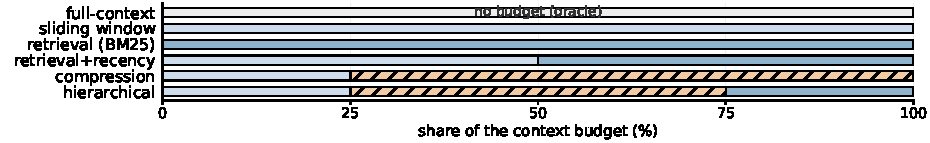
\includegraphics[width=0.88\textwidth]{tables/fig_policy_anatomy.pdf}
\caption{Budget allocation of the six families. Light blue: most recent turns; medium blue:
BM25-retrieved verbatim turns; hatched: LLM session digests; grey: full context, which
ignores the budget. Each budgeted policy spends a fixed mix of the three tiers; the grid
varies this mix, not the tier contents.}
\label{fig:anatomy}
\end{figure}

\paragraph{Retriever configuration.} BM25 uses the Okapi implementation (rank-bm25) with
library defaults $k_1{=}1.5$, $b{=}0.75$, tokenizing each turn on whitespace
\citep{robertson2009bm25}; there is \emph{no fixed top-$k$}: the per-question retrieval
cutoff is the budget itself---turns are admitted in descending BM25 score until the
context fills, so larger budgets strictly widen the candidate set. The dense ablation
embeds turns and questions with the local bge-small-en-v1.5 encoder (384-d, CPU) and ranks
by cosine similarity with the standard bge query prefix; the hybrid ablation fuses the
BM25 and dense rankings by reciprocal-rank fusion ($k{=}60$). All retrievers share the
same turn granularity and chronological re-injection order, so differences isolate the
ranking rule.

\paragraph{Real-LLM summarization.} For every unique haystack session ($19{,}195$
across our sample) we generate one fact-dense digest ($\leq$60 words: names, dates,
numbers, preferences, decisions) with the same answerer model, greedy decoding. Digests
are cached by session id and reused across questions and budgets; summaries of the same
session are identical for the compression and hierarchical policies, so the write-side
cost is one-shot and amortized across all 25 cells.

\paragraph{Structured compressor variants.} To separate \emph{format} from \emph{lossiness},
two structured compressors run under the identical 60-word cap, greedy decoding, and frozen
cache: \textbf{KV} extracts label--value fact lines copied verbatim, \textbf{EDU} atomic
discourse units copied verbatim. Both reuse the compression assembly unchanged (25\% recency
$+$ 75\% compressed tier), so any effect is bounded to \emph{reading} (\S\ref{sec:reading}).

\paragraph{Answerers and readers.} The \emph{primary} answerer is DeepSeek-V4.1-Flash
(greedy, temperature $0$, max 64 output tokens), used for all 25 main-grid cells at
$n{=}500$ and for the per-session digests. Three additional readers test robustness on the
same harness and the same question pool: (i)~\textbf{mimo-v2.6-flash} re-runs the entire
21-cell grid on the stratified $120$-question subset with its own digests (the original
generation of the study); (ii)~\textbf{GLM-4-Flash} re-runs the same 21-cell grid on the
same subset, likewise with its own digests (Appendix~\ref{app:secondreader}); and
(iii)~a \textbf{frozen-artifact probe} re-answers a $60$-question subset with
GLM-4.7-Flash (thinking disabled) over memory artifacts frozen from the GLM-4-Flash tier,
isolating the reader from the memory artifacts. The full-set claims rest on the primary
reader; the three others are robustness checks and are never pooled with the main grid.
The primary reader is not the highest-scoring one on the shared subset (retrieval@4096:
$0.375$ vs.\ mimo $0.408$), so no claim here rests on it being ``strongest''---it is the
reader for which the complete $500$-question grid was obtainable after the original
mid-scale gateway was retired.

\paragraph{Answering and scoring.} Each policy's memory context is wrapped in a fixed
instruction template (reproduced verbatim in Appendix~\ref{app:template}) and answered by
the reader at temperature $0$. We report three deterministic scores computed after a
shared normalization (lower-casing, punctuation stripping, article removal, whitespace
folding): \textbf{EM}, exact equality of the normalized strings; \textbf{EM$_{\text{rel}}$}
(relaxed EM), which scores 1 when the normalized gold string is a \emph{substring} of the
normalized prediction, tolerating minor padding (e.g., ``5 painting projects'' vs.\ gold
``5''); and \textbf{token-F1}, token-overlap F1. Headline comparisons use
EM$_{\text{rel}}$ (SQuAD-style containment); \S\ref{sec:frontier} reports all three. No
LLM judge enters the headline metrics, avoiding judge-model circularity; a semantic judge
appears only as a robustness check with correct-answer controls (\S\ref{sec:reading}).

\paragraph{Statistics and power.} All comparisons are \emph{per-question paired}: bootstrap
95\% CIs (10{,}000 resamples, seed 42) on accuracy differences and exact McNemar tests.
Compression is tested against a \emph{dual baseline}: BM25 retrieval (verbatim, like-for-like)
plus the strongest non-compression alternative at each budget. Greedy decoding makes
single-run results deterministic per question. With $n{=}500$ the observed discordant counts
give exact $p<10^{-4}$ for compression-vs-retrieval at $512$--$2048$, and the CI half-width
on accuracy differences is $0.02$--$0.04$, bounding the minimum detectable effect at roughly
$0.04$ EM. Within a question type ($n{=}56$--$133$) the paired CI half-width is
$0.05$--$0.08$ EM, so type-level contrasts are tested rather than merely described. All
tables name their answering reader; absolute numbers compare \emph{within-table} only.

\paragraph{What is directly comparable.} Because the study spans one full-set grid and several
probe runs, Table~\ref{tab:map} states, for each table, its question set, reader and the
comparisons it supports: main-grid rows are mutually paired at every budget, probe tables are
paired only against their own baseline.

\begin{table}[h]
\centering\scriptsize
\caption{Comparability map. ``Full'' = all 500 questions; ``sub'' = stratified 120-question
subset (seed 42). A dash means the run does not cover that budget. \emph{Within} means
paired comparisons are valid inside the table only.}
\label{tab:map}
\setlength{\tabcolsep}{2pt}
\begin{tabular}{lllccl}
\toprule
Table & Question set & Reader & Budgets & Comparable \\
\midrule
Main grid (\ref{tab:main}), stats (\ref{tab:stats}), by type (\ref{tab:bytype})
  & full ($n{=}500$) & DeepSeek-V4.1-Flash & $512$--$4096$ & within, all cells paired \\
Cost profile (\ref{tab:latency}) & sub ($n{=}30$) & DeepSeek-V4.1-Flash & $4096$ & within, single stream \\
Reranker / format probes (text) & sub ($n{=}120$) & GLM-4.7-Flash & $4096$ & within only \\
Ablations (\ref{tab:ablations}), plug-ins (\ref{tab:plugin}) & sub ($n{=}120$) & GLM-4.x probe & $512$--$4096$ & within only \\
Cross-reader (\ref{tab:reader}) & full / sub & four readers & $4096$ & matched questions only \\
Order / template probe (App.~\ref{app:rebuttal}) & sub ($n{=}120$) & GLM-4.7-Flash & $4096$ & within only \\
Tight budgets (\ref{tab:tight}), stronger families (\ref{tab:probes}) & sub / full & DeepSeek-V4.1 & $64$--$4096$ & within only \\
\bottomrule
\end{tabular}
\end{table}

\paragraph{Latency definitions.} We report (i)~\emph{memory-access latency}: wall time of
policy context assembly including BM25 scoring, measured offline over all $500$ questions, and
(ii)~\emph{end-to-end latency}: the full answer API call including the LLM forward pass,
measured in a single-stream calibration. The two are reported separately, never mixed.
Window/compression assembly is an $O(1)$ slice plus cached-digest lookup (no scoring), hence
$0.1$--$4$\,ms access at any size; retrieval-family policies score every turn with BM25
($27$--$55$\,ms)---a mechanism-family property (the trilemma's latency axis), not an artifact.
Monetary cost is linear in the same footprint: full-context consumes ${\sim}104$k prompt
tokens per question vs.\ ${\sim}4$k at $B{=}4096$---a provider-independent $25\times$
per-question cost ratio, so at any posted per-token price the budgeted frontier is an order
of magnitude cheaper.

\paragraph{Provider-side failures (archived generation).} An earlier full-context sweep under
a different reader suffered a rate-limit storm that left client-layer empty calls, and four
questions triggered deterministic input-side content-filter refusals whenever the offending
turn entered the context. Those records are retained in \texttt{results\_archive.jsonl},
scored as they stand, and are never pooled with the main grid. The primary grid has no empty
prediction and no refusal (\fcDoneN{} full-context calls, all delivered).

\paragraph{Infrastructure.} All calls go through the OpenAI-compatible endpoint configured
for the answerer model, shared with the JiuwenSwarm framework configuration; per-call
usage (prompt/completion tokens) and latencies are logged per question and aggregated by
script. The harness, records, and aggregation scripts are released for reproduction;
\texttt{pytest} on the offline suite gives 69 passed / 1 skipped, and the deterministic
sandbox run reports \texttt{deterministic: true}.

\section{The Accuracy--Cost--Latency Frontier}
\label{sec:frontier}
\subsection{Main comparison}
Table~\ref{tab:main} reports EM, relaxed EM, and token-F1 per policy and budget, and
Figure~\ref{fig:takeaway} plots the relaxed-EM trajectory with per-cell bootstrap 95\% CIs;
the remaining tables disaggregate by latency and footprint, paired statistics, and question
type. All cells are $n{=}\longmemN{}$ with zero empty predictions.

\begin{table}[h]
\centering\scriptsize
\caption{Main grid (primary reader DeepSeek-V4.1-Flash, full 500-question set): EM,
relaxed EM (EM$_{\text{rel}}$), and token-F1 per cell, reproduced verbatim from the
released records (\texttt{tables500/main.tex}). Twenty-five cells: six families, with the
compression family run in write-time and read-time variants that differ only in how the
digest tier is filled. $^{\dagger}$Full-context has no budget and
is a lossless oracle reference, not a deployable policy. Every cell is an all-question mean
over $n{=}500$ delivered calls; no cell has an empty prediction.}
\label{tab:main}
\setlength{\tabcolsep}{2.5pt}
\begin{tabular}{@{}llcccc@{}}
\toprule
Policy & $B$ & $n$ & EM & EM$_{\text{rel}}$ & F1 \\
\midrule
full-context$^{\dagger}$ & -- & 500 & 0.3420 & 0.3700 & 0.4651 \\
window & 512 & 500 & 0.0360 & 0.0360 & 0.0668 \\
window & 1024 & 500 & 0.0440 & 0.0540 & 0.0761 \\
window & 2048 & 500 & 0.0440 & 0.0560 & 0.0804 \\
window & 4096 & 500 & 0.0580 & 0.0680 & 0.0991 \\
retrieval & 512 & 500 & 0.2500 & 0.2720 & 0.3494 \\
retrieval & 1024 & 500 & 0.2940 & 0.3120 & 0.3900 \\
retrieval & 2048 & 500 & 0.3120 & 0.3340 & 0.4121 \\
retrieval & 4096 & 500 & 0.3400 & 0.3640 & 0.4457 \\
retr.+recency & 512 & 500 & 0.2500 & 0.2740 & 0.3428 \\
retr.+recency & 1024 & 500 & 0.2680 & 0.2880 & 0.3625 \\
retr.+recency & 2048 & 500 & 0.2880 & 0.3100 & 0.3869 \\
retr.+recency & 4096 & 500 & 0.3200 & 0.3420 & 0.4273 \\
\bottomrule
\end{tabular}~~%
\begin{tabular}{@{}llcccc@{}}
\toprule
Policy & $B$ & $n$ & EM & EM$_{\text{rel}}$ & F1 \\
\midrule
compr. (write) & 512 & 500 & 0.1160 & 0.1240 & 0.1732 \\
compr. (write) & 1024 & 500 & 0.1560 & 0.1720 & 0.2211 \\
compr. (write) & 2048 & 500 & 0.2160 & 0.2420 & 0.3076 \\
compr. (write) & 4096 & 500 & 0.2860 & 0.3340 & 0.3992 \\
compr. (+read) & 512 & 500 & 0.2180 & 0.2620 & 0.3295 \\
compr. (+read) & 1024 & 500 & 0.2540 & 0.2920 & 0.3722 \\
compr. (+read) & 2048 & 500 & 0.2800 & 0.3180 & 0.3873 \\
compr. (+read) & 4096 & 500 & 0.2800 & 0.3240 & 0.4131 \\
hierarch. & 512 & 500 & 0.1860 & 0.2080 & 0.2639 \\
hierarch. & 1024 & 500 & 0.2380 & 0.2680 & 0.3285 \\
hierarch. & 2048 & 500 & 0.3040 & 0.3280 & 0.4114 \\
hierarch. & 4096 & 500 & 0.3440 & 0.3720 & 0.4639 \\
\bottomrule
\end{tabular}
\end{table}

% Table 3 (consolidated grid) is replaced by Figure 2

\begin{figure}[h]
\centering
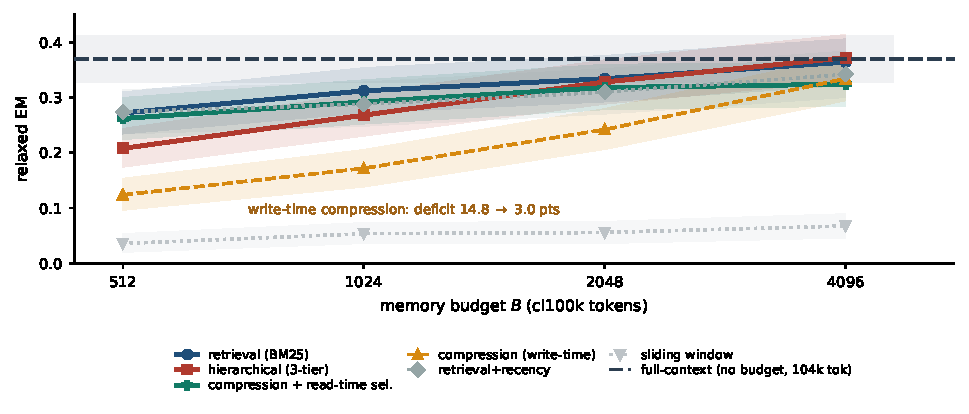
\includegraphics[width=0.82\textwidth]{tables/fig_takeaway.pdf}
\caption{Main-grid accuracy vs.\ budget (primary reader, $n{=}500$ per cell; bands: per-cell
95\% bootstrap). Dashed: full-context reference. Retrieval is best or tied-best up to $2048$;
hierarchy draws level at $4096$; write-time compression closes from $14.8$ to $3.0$ points
without leading, while read-time selection tracks retrieval at $512$--$2048$.}
\label{fig:takeaway}
\end{figure}

\textbf{Full-context buys no accuracy over the best budgeted policy.} Its $0.370$ relaxed EM
($104$k memory tokens, $5.8$\,s per question single-stream, \S\ref{sec:cost}) is statistically
indistinguishable from the $4$k-token hierarchical engine ($0.372$; $\Delta{=}-0.002$, CI
$[-0.036,+0.032]$, exact McNemar $p{=}1.0$, $42$ vs.\ $43$ flips). At $25\times$ the footprint
this is a reference point, not a policy.
\textbf{Among budgeted strategies the leader is budget-conditioned:} BM25 retrieval is best or
tied-best at $512$--$2048$ ($0.272/0.312/0.334$), the hierarchical engine rises monotonically
($0.208 \rightarrow 0.268 \rightarrow 0.328 \rightarrow 0.372$; $4096$ vs.\ $2048$
$\Delta{=}+0.044$, relaxed-EM $p{=}0.005$) and draws level at $4096$ ($0.372$ vs.\ $0.364$,
$\Delta{=}-0.008$, $p{=}0.90$). \textbf{Compression's deficit depends on how its digests are
read.} Write-time compression climbs from $0.124$ at $512$ to $0.334$ at $4096$; its gap to
retrieval narrows from $14.8$ to $3.0$ points, significant at $512$--$2048$ ($p<10^{-4}$) but
not at $4096$ under the headline metric ($p{=}0.15$; strict EM $p{=}0.009$). Selecting digests
by relevance at read time removes
most of it at small budgets: $0.262/0.292/0.318$ vs.\ $0.272/0.312/0.334$ for retrieval
($p{=}0.70/0.36/0.50$), and $0.324$ vs.\ $0.364$ at $4096$ ($\Delta{=}-0.040$, $p{=}0.059$).
Read-time selection thus ties retrieval at three of four budgets at a few milliseconds of
assembly per question (\S\ref{sec:cost}): the write-time deficit is a design choice, not a
property of compression. Sliding window stays near floor ($0.036$--$0.068$).

\subsection{Cost profile}
\label{sec:cost}
Table~\ref{tab:latency} reports memory-access latency (median over $500$ assemblies, measured
offline with no model calls) and mean memory footprint per cell.

\begin{table}[h]
\centering\scriptsize
\caption{Memory-access latency (ms; median over the $500$ assemblies) and memory footprint
(tokens; mean) per policy and budget, primary reader. End-to-end latency is measured
separately in a single-stream calibration (text). Source \texttt{tables500/latency.tex}.}
\label{tab:latency}
\begin{tabular}{llcc}
\toprule
Policy & Budget & access (ms) & mem.\ tokens \\
\midrule
full-context (verbatim)$^{\dagger}$ & -- & 32.94 & 104024 \\
sliding window & 512 & 0.10 & 333 \\
sliding window & 1024 & 0.22 & 826 \\
sliding window & 2048 & 0.50 & 1809 \\
sliding window & 4096 & 1.10 & 3897 \\
retrieval (BM25) & 512 & 29.68 & 300 \\
retrieval (BM25) & 1024 & 28.10 & 848 \\
retrieval (BM25) & 2048 & 30.09 & 1861 \\
retrieval (BM25) & 4096 & 30.92 & 3842 \\
retrieval+recency & 512 & 27.26 & 334 \\
retrieval+recency & 1024 & 28.34 & 828 \\
retrieval+recency & 2048 & 30.37 & 1843 \\
retrieval+recency & 4096 & 36.71 & 3875 \\
compression (write-time) & 512 & 0.49 & 471 \\
compression (write-time) & 1024 & 0.91 & 985 \\
compression (write-time) & 2048 & 2.42 & 2007 \\
compression (write-time) & 4096 & 4.22 & 4038 \\
hierarchical (3-tier) & 512 & 51.77 & 284 \\
hierarchical (3-tier) & 1024 & 54.44 & 686 \\
hierarchical (3-tier) & 2048 & 52.32 & 1614 \\
hierarchical (3-tier) & 4096 & 47.49 & 3683 \\
\bottomrule
\end{tabular}
\end{table}

Access time separates the families cleanly: sliding window costs $0.1$--$1.1$\,ms,
compression $0.5$--$4.2$\,ms, and the retrieval family $27$--$55$\,ms (BM25 over roughly
fifty sessions per question). Footprint is the budget by construction ($300$--$4{,}000$
tokens), except full-context at $104$k. The trilemma is visible on these two axes alone: the
policies that answer in milliseconds are exactly the ones that lose accuracy, and the ones
that win accuracy pay two orders of magnitude more access time. End-to-end, however, the
reader call dominates every policy (single-stream calibration, $n{=}30$ at $B{=}4096$:
\eTwoERange{}), so access-time differences are invisible to a user and only the token
footprint changes the bill. That is the axis on which full-context loses: it buys no
accuracy for $25\times$ the tokens.

\paragraph{Write-side accounting.} Comparisons above are answer-side; the one-time
construction cost of write-time digests completes the trilemma. Digest generation averaged
$2{,}849$ tokens per session ($54.7$M tokens for all $19{,}195$ sessions, $\approx$4\,h
wall-clock for the summary pass, primary reader); a freshly-digested question draws $20.1$
sessions on average, i.e.\ \approx$57\,k$ tokens of one-time write---about
$14\times$ the largest read budget. Once built, digests are frozen and reused across questions
and cells, and read-side cost is at parity with retrieval ($4{,}197$ vs.\ $3{,}989$ mean
prompt tokens at $B{=}4096$). Retrieval, hierarchical and full-context incur zero LLM write
cost, and the structured verbatim compressors are deterministic. Deployments where write
time is non-negligible should bill this pass separately: it is the cheapest-to-read family
that pays the largest one-time write.

\subsection{Statistical tests}
Table~\ref{tab:stats} reports, per budget, the paired bootstrap 95\% CI and the exact McNemar
$p$-value for the write-time compression policy under the dual-baseline protocol---computed
separately under \emph{both} metrics. The two agree at $512$--$2048$: compression trails
retrieval by $-0.148$, $-0.140$, $-0.092$ relaxed EM points ($p<10^{-4}$; strict EM
$-0.134/-0.138/-0.096$, same verdict). At $4096$ they diverge, and we report the divergence
rather than one of its sides: the relaxed-EM gap is $-0.030$ (CI $[-0.068,+0.008]$,
$p{=}0.146$), the strict-EM gap $-0.054$ (CI $[-0.092,-0.016]$, $p{=}0.009$). We therefore
describe $4096$ as a \emph{narrowing} gap, not a proven deficit. The same holds against
hierarchical at $4096$ (strict $p{=}0.004$, relaxed $p{=}0.050$, CI $[-0.074,-0.002]$). A
direct paired comparison of the two leading policies at $4096$ gives retrieval vs.\
hierarchical $\Delta{=}-0.008$ $[-0.038,+0.024]$, exact McNemar $p{=}0.905$ ($34$ vs.\
$36$ discordant flips): the hierarchical edge is within noise, so we say the two
\emph{draw level}, not that one overtakes the other. Hierarchical's own scaling step from
$2048$ to $4096$ is significant ($+0.044$, relaxed $p{=}0.005$; strict $p{=}0.015$), as is
retrieval's ($+0.030$, $p{=}0.060$, borderline); the difference between the two curves is not.
The read-time compression variant is tested against the same baselines: it is statistically
indistinguishable from retrieval at $512$--$2048$ ($p{=}0.70/0.36/0.50$) and $4.0$ points
below at $4096$ ($p{=}0.059$).

\begin{table}[h]
\centering\scriptsize
\caption{Per-budget paired statistics for the write-time compression policy, reported
separately under strict EM (left) and relaxed EM (right); $\Delta$ is compression minus
baseline, so negative means compression is worse. The two metrics agree at $512$--$2048$ and
diverge at $4096$. Primary comparison against BM25 retrieval; the strongest non-compression
alternative at $4096$ appears as a second row. Source \texttt{tables500/stats.tex}.}
\label{tab:stats}
\setlength{\tabcolsep}{2.5pt}
\begin{tabular}{llcccccc}
\toprule
 & & \multicolumn{3}{c}{strict EM} & \multicolumn{3}{c}{relaxed EM} \\
\cmidrule(lr){3-5}\cmidrule(lr){6-8}
Budget & Baseline & $\Delta$ & 95\% CI & McNemar $p$ & $\Delta$ & 95\% CI & McNemar $p$ \\
\midrule
512 & retrieval (BM25) & -0.1340 & [-0.176, -0.092] & 0.0000 & -0.1480 & [-0.190, -0.106] & 0.0000 \\
1024 & retrieval (BM25) & -0.1380 & [-0.180, -0.094] & 0.0000 & -0.1400 & [-0.182, -0.096] & 0.0000 \\
2048 & retrieval (BM25) & -0.0960 & [-0.138, -0.054] & 0.0000 & -0.0920 & [-0.132, -0.052] & 0.0000 \\
4096 & retrieval (BM25) & -0.0540 & [-0.092, -0.016] & 0.0086 & -0.0300 & [-0.068, +0.008] & 0.1462 \\
4096 & hierarchical (3-tier) & -0.0580 & [-0.096, -0.020] & 0.0038 & -0.0380 & [-0.074, -0.002] & 0.0503 \\
\bottomrule
\end{tabular}
\end{table}

\subsection{Accuracy by question type}
Table~\ref{tab:bytype} disaggregates strict EM by question-type family on the full set
(per-type $n$: $70$ single-user, $56$ single-assistant, $30$ single-preference, $133$
multi-session, $133$ temporal, $78$ knowledge-update).

\begin{table}[h]
\centering\scriptsize
\caption{Strict EM by question-type family (all budgets pooled per policy; full-context from
its single run; $n{=}500$). Single-preference questions are open-ended and score $0.000$ for
every policy under exact match, so the three single-session types are pooled. Source
\texttt{tables500/bytype.tex}.}
\label{tab:bytype}
\begin{tabular}{lccccc}
\toprule
Policy & single-* & multi & temporal & update & overall \\
\midrule
full-context (verbatim)$^{\dagger}$ & 0.519 & 0.248 & 0.143 & 0.487 & 0.342\\
sliding window & 0.029 & 0.000 & 0.096 & 0.071 & 0.045\\
retrieval (BM25) & 0.460 & 0.171 & 0.115 & 0.510 & 0.299\\
retrieval+recency & 0.438 & 0.148 & 0.107 & 0.494 & 0.281\\
compression (write-time) & 0.229 & 0.105 & 0.113 & 0.410 & 0.194\\
hierarchical (3-tier) & 0.389 & 0.158 & 0.113 & 0.478 & 0.268\\
\bottomrule
\end{tabular}
\end{table}

\begin{itemize}\setlength{\itemsep}{1pt}
\item \textbf{Every budgeted strategy collapses on multi-session and temporal questions:}
multi-session $\leq 0.171$ vs.\ full-context $0.248$; temporal $\leq 0.115$ vs.\ $0.143$---
the cross-session composition and time-ordering the retrieval family misses most.
\item \textbf{Compression is weakest on knowledge-update} among non-window strategies
($0.410$ vs.\ retrieval $0.510$ and full-context $0.487$; $n{=}78$), consistent with
write-time summaries evicting superseded values.
\item Retrieval \emph{matches} full-context on knowledge-update questions ($0.510$ vs.\
$0.487$), indicating update questions are easy when evidence is localized.
\item \textbf{No type-level difference between the two leaders survives the full set:}
paired retrieval vs.\ hierarchical at $4096$ gives $\Delta{=}+0.014$ (single-user),
$+0.036$ (single-assistant), $-0.053$ (multi-session), $-0.023$ (temporal) and $+0.038$
(knowledge-update), with exact McNemar $p \geq 0.26$ throughout and per-type CI half-widths
of $0.05$--$0.08$ EM. The family-level ordering is a budget effect, not a type effect.
\end{itemize}

egin{table}[h]
\centering\scriptsize
\caption{Per-type, per-budget paired comparison, hierarchical minus retrieval (relaxed EM,
exact McNemar; $^{**}p{<}0.01$, $^{*}p{<}0.05$; primary reader, full set). The significant
retrieval edge lives at small budgets and on single-session / multi-session questions; from
$B{=}2048$ on, no family differs significantly and multi-session / temporal tilt (n.s.)\ toward
hierarchical at $4096$. Source 	exttt{tables500/type\_paired.tex}
(regenerated by 	exttt{type\_paired.py} from 	exttt{results.jsonl}).}
\label{tab:typepaired}
\begin{tabular}{lccccc}
\toprule
Family & $B{=}512$ & $B{=}1024$ & $B{=}2048$ & $B{=}4096$ & pooled \\
\midrule
single-* ($n{=}156$/budget) & $-0.115$** & $-0.058$ & $-0.038$ & $-0.019$ & $-0.058$** \\
multi-session ($n{=}133$) & $-0.075$* & $-0.068$ & $+0.023$ & $+0.053$ & $-0.017$ \\
temporal ($n{=}133$) & $-0.008$ & $-0.015$ & $+0.008$ & $+0.023$ & $+0.002$ \\
knowledge-update ($n{=}78$) & $-0.038$ & $-0.026$ & $-0.013$ & $-0.038$ & $-0.029$ \\
overall ($n{=}500$) & $-0.064$** & $-0.044$* & $-0.006$ & $+0.008$ & $-0.027$** \\
\bottomrule
\end{tabular}

\end{table}

Table~
ef{tab:typepaired} adds the budget dimension to the pairing. Retrieval's overall
edge is a small-budget effect ($-0.064^{**}$ at $512$) concentrated in single-session
($-0.115^{**}$) and multi-session ($-0.075^{*}$) questions; it decays monotonically and no
family differs significantly from $B{=}2048$ on, with hierarchical numerically ahead on
multi-session ($+0.053$) and temporal ($+0.023$) at $4096$. Practitioners can condition on
workload composition: single-session-heavy traffic favors retrieval at every budget;
multi-session/temporal-heavy traffic reaches parity by $2048$ and tilts (n.s.)\ toward the
hierarchy at $4096$.

\section{Why No Strategy Dominates: Mechanistic Readings}
\label{sec:mechanism}
The frontier of \S\ref{sec:frontier} shows \emph{that} no strategy wins on all three
axes; this section explains \emph{why}, with four mechanistic readings grounded in the
same records.

\paragraph{C1 --- Digests displace verbatim evidence at small budgets.} Each
$\sim$80-token session digest displaces several verbatim turns that BM25 would otherwise
surface exactly. Compression's token-F1 does scale with budget ($0.173 \rightarrow
0.399$) as more digests fit, but it does not catch retrieval's verbatim recall early in
the grid: summary compression changes fact presentation, which hurts exact answer
matching on single-fact questions. \emph{Evidence:} compression's gap to BM25 retrieval is
largest at $512$ ($\Delta{=}-0.148$ relaxed EM, CI $[-0.190,-0.106]$) and narrows at $4096$ to
$-0.030$ (CI $[-0.068,+0.008]$; strict-EM $p{=}0.009$, relaxed $p{=}0.15$, so the point
estimate narrows but the relaxed-EM deficit is no longer resolvable at $n{=}500$); the per-cell
trajectory is plotted in Figure~\ref{fig:takeaway}. Reading digests by relevance instead of
recency recovers most of the small-budget gap (\S\ref{sec:frontier}), which sharpens the
reading: the loss is partly \emph{which} digests are shown, not only that digests are shown.

\paragraph{C2 --- Full-context: no accuracy premium, and fragile delivery.} Full-context
injects $\sim$104k tokens. In the primary run all $500$ calls delivered, reaching $0.370$
relaxed EM---statistically identical to the $4$k-token hierarchical engine ($0.372$) and
$0.006$ above BM25 retrieval ($p{=}1.0$ for both). Its prompts cost about twice the
single-stream wall-clock, and an archived sweep under a different reader suffered a rate-limit
storm that left client-layer empty calls. A $4$k-token retrieval window preserves all of the
accuracy at $4\%$ of the footprint; under mimo the same comparison favoured full-context by
$0.058$, the reader dependence quantified in \S\ref{sec:crossreader}.

\paragraph{C3 --- Hybrid tiers keep scaling where single-mechanism leaders flatten.}
Retrieval rises across the grid but decelerates after $1024$ ($0.312 \rightarrow 0.334
\rightarrow 0.364$); retrieval+recency stays below pure retrieval at \emph{every} budget
($0.274/0.288/0.310/0.342$ vs.\ $0.272/0.312/0.334/0.364$), because the recency half
fills with low-value recent turns. Only hierarchical keeps rising steeply
($0.208 \rightarrow 0.268 \rightarrow 0.328 \rightarrow 0.372$) and draws level with
retrieval at $4096$: splitting the budget across complementary tiers is associated with
continued scaling where each single-mechanism leader flattens.

\paragraph{C4 --- Memory access is not the end-to-end bottleneck.} BM25 scoring costs tens
of milliseconds; the answer forward pass costs seconds. Latency claims about memory policies
must be component-separated: assembling the context is invisible next to the reader call, so
optimizing it (e.g., dropping BM25 for a take-newest store) trades away accuracy for a saving
no user observes.

\section{Where the Residual Error Lives}
\label{sec:reading}
A natural objection is that constrained policies fail simply because the evidence never
reaches the context. This section tests that objection at three granularities---session,
turn, and reader---with a failure decomposition, a ranking audit, two oracle injections, a
reranker intervention, and a format control. The answer is not a single stage: session
retrieval is essentially solved, turn-level selection is not, and even a distractor-free
evidence context leaves most residual errors in place.

\subsection{Session, turn, and reader: a three-way decomposition}
\label{sec:diag}
We separate the stages using the \emph{gold session} labels of LongMemEval-S:
re-running each policy's memory assembly offline, we record whether any retained turn or
digest originates from a gold session (\emph{gold recall}) and cross-tabulate it with
correctness (Table~\ref{tab:diag}). A question whose gold evidence is present yet answered
wrong is a \emph{session-level read} failure; one whose evidence never arrives is a
\emph{retrieval} failure. Both are computed on the full $500$-question grid.

\begin{table}[h]
\centering\scriptsize
\caption{Failure localization on the full grid ($n{=}500$; two operating points per policy).
\emph{gold recall}: share of questions whose gold session reaches the context;
\emph{acc$|_{\mathrm{covered}}$}: accuracy restricted to those questions;
\emph{read-fail}/\emph{retr.-fail}: shares of \emph{all} questions failing with and without
gold-session coverage (they sum with accuracy to one). Source
\texttt{tables500/diag.tex}.}
\label{tab:diag}
\begin{tabular}{llcccc}
\toprule
Policy & Budget & gold recall & acc$|_{\mathrm{covered}}$ & read-fail & retr.-fail \\
\midrule
sliding window & 1024 & 0.050 & 0.200 & 0.040 & 0.906 \\
sliding window & 4096 & 0.104 & 0.250 & 0.078 & 0.854 \\
retrieval (BM25) & 1024 & 0.880 & 0.352 & 0.570 & 0.118 \\
retrieval (BM25) & 4096 & 0.968 & 0.374 & 0.606 & 0.030 \\
retrieval+recency & 1024 & 0.844 & 0.337 & 0.560 & 0.152 \\
retrieval+recency & 4096 & 0.940 & 0.362 & 0.600 & 0.058 \\
compression & 1024 & 0.462 & 0.342 & 0.304 & 0.524 \\
compression & 4096 & 0.958 & 0.347 & 0.626 & 0.040 \\
hierarchical & 1024 & 0.736 & 0.356 & 0.474 & 0.258 \\
hierarchical & 4096 & 0.962 & 0.387 & 0.590 & 0.038 \\
\bottomrule
\end{tabular}
\end{table}

The pattern is unambiguous at the session level. At $4096$ tokens BM25 delivers the gold
session for $96.8\%$ of questions, yet accuracy among covered questions is only $0.374$:
session retrieval fails on $3.0\%$ of questions, while $60.6\%$ fail \emph{after the gold
session is in context}. Hierarchical and compression show the same signature (gold recall
$0.962$/$0.958$; read-fail $0.590$/$0.626$), and only the sliding window fails
predominantly at retrieval ($0.854$). Before truncation the ranker is already strong: BM25
places a gold session at Recall@$1$ $0.728$, @$5$ $0.898$ and @$10$ $0.952$ over all $500$
questions; on the $120$-question probe the dense and hybrid rankers reach R@$5$
$0.968$/$0.947$, and only recency ordering fails ($0.111$).

Session coverage is nevertheless an \emph{upper bound} on reading failure: a gold session
can enter the context without the turn that carries the answer. A turn-level audit of the
$303$ covered-but-wrong questions at $4096$ locates the answer-bearing turn inside the
injected context for $25.1\%$, only in the unconsumed history for $49.5\%$, and nowhere for
$25.4\%$ (paraphrastic or aggregate golds)---$15.2\%$/$30.0\%$/$15.4\%$ of all $500$
questions. The concern that session-level labels over-attribute to reading is therefore
quantitatively right: the $60.6\%$ is not all reading.

Two oracle injections bound what the residual is. Re-asking each covered-but-wrong question
over \emph{all turns of its gold sessions and nothing else}---no distractors---fixes $46$ of
$303$ ($15.2\%$, CI $[11.2,19.1]$); with the context capped at $4096$ tokens it fixes $38$
($12.5\%$), so truncation is not the driver. Re-asking with only the located bearing turn
fixes $24$ of $226$ ($10.6\%$). Removing distractors and repairing turn selection thus
recover little: $85\%$ of covered failures survive a clean, evidence-only context. The
residual is compositional reasoning over several turns---multi-session ($100$ of $303$) and
temporal ($108$ of $303$) questions dominate---which this reader cannot perform and no
ranking improvement can supply.

This also reconciles our result with retrieval-dominant studies, which we read as a
difference in regime rather than in findings. Extending the grid downward
(Table~\ref{tab:tight}), retrieval failures dominate at $64$ tokens (gold recall $0.225$;
retr.-fail $0.725$), are balanced at $128$--$256$ ($0.542$/$0.417$ and $0.600$/$0.375$), and
are outweighed by read failures from $512$ on ($0.817$ vs.\ $0.158$). Which stage binds is a
function of the budget: below roughly $256$ tokens the evidence does not arrive; above it the
reader cannot use what arrives.

\textbf{Implication:} at $\geq 512$ tokens, effort should move from \emph{finding} sessions
to \emph{composing} answers from the turns already present---selection, ordering, and
aggregation---rather than to a larger $k$.

\begin{table}[h]
\centering\scriptsize
\caption{Tiny-budget regime (stratified $120$-question subset, same reader): relaxed EM at
$64/128/256$ tokens, with the $512$ cell of the main grid for reference. Failure
decomposition for these cells is given in the text. Source \texttt{tables500/tight.tex}.}
\label{tab:tight}
\begin{tabular}{lcccc}
\toprule
Policy & $B{=}64$ & $B{=}128$ & $B{=}256$ & $B{=}512$ \\
\midrule
retrieval (BM25) & 0.092 & 0.158 & 0.225 & 0.308\\
compression & 0.050 & 0.042 & 0.083 & 0.100\\
hierarchical & 0.042 & 0.058 & 0.092 & 0.200\\
\bottomrule
\end{tabular}
\end{table}

\subsection{Ranking or reading? A reranker probe at fixed budget}
\label{sec:rerank}
The post-2048 deceleration could reflect mediocre ranking (fixable by a better retriever)
or a read-side ceiling. We re-rank the BM25 and dense (bge-base) top-50 candidates with a
local cross-encoder (bge-reranker-base, CPU) and re-answer under the \emph{same} budgets
and answerer. The probe shows the dissociation: the reranker lifts offline
session Recall@5 from $0.834$ to $0.954$ (BM25) and $0.969$ to $0.981$ (dense), yet online
relaxed EM at $4096$ is unchanged---BM25 $\Delta{=}-0.008$ (exact McNemar $p{=}1.0$),
dense-rerank $\Delta{=}0.000$ ($p{=}1.0$); the encoder upgrade itself adds a
non-significant $+0.025$ ($p{=}0.55$). It re-orders \emph{sessions}---a stage already at
$0.97$ recall---and leaves turn-level selection unchanged, so the null result is consistent
with the decomposition above. Serving cost independently rules it out
online: the cross-encoder adds a mean $15.5$\,s per question on CPU---$3.6\times$ the
entire answer call---versus $35$\,ms for BM25 scoring, so it is a diagnostic tool, not a
deployable stage.


\subsection{Is it the format? Structured verbatim compressors}
\label{sec:struct}
A natural defense of compression is that \emph{free-form} paraphrase is the problem: a
structured digest that copies facts verbatim should preserve answer strings. We test this
with the two preregistered structured compressors of \S\ref{sec:design} (KV and EDU, both
verbatim) under the identical 60-word cap, budget, assembly, and answerer, with the
free-form w60 digest as control. The preregistered judgment is the \emph{gap-closed ratio}
at $B{=}4096$: $(\text{struct}-\text{freeform})/(\text{BM25}-\text{freeform})$, with tiers
$<20\%$ / $20$--$60\%$ / $\geq 60\%$. The verdict is: KV closes
$-11.8\%$ of the gap (slightly \emph{worse} than free-form, $0.142$ vs.\ $0.158$); EDU
closes $0.0\%$ ($0.158$, identical to free-form). Both fall in the strongest-negation
tier: \emph{in this setting, lossy compression without query-time selection failed as a
standalone policy regardless of digest format}---though \S\ref{sec:ablation} shows that
selecting digests by relevance at read time recovers much of the gap at $1024$ tokens. These are diagnostic runs compared \emph{within-run} only.


\section{Robustness: Sensitivity Analyses and Cross-Reader Replication}
\label{sec:robust}
\subsection{Sensitivity ablations}
\label{sec:ablation}
Four follow-up experiments probe the robustness of the headline findings
(Table~\ref{tab:ablations} and \ref{tab:plugin}); a fifth tests the hierarchy family under a
stronger retrieval design (Table~\ref{tab:probes}).

\textbf{Summarizer length (Table~\ref{tab:ablations}a).} Longer digests help at $4096$
($0.117 \rightarrow 0.156 \rightarrow 0.200$ for 20/60/120 words) but stay below retrieval,
and the 120-word variant dips below 60 at $\leq 2048$: the deficit is not a granularity
artifact. \textbf{Tier allocation (Table~\ref{tab:ablations}b).} Moving the $25/50/25$ split to
$15/70/15$ or $40/20/40$ leaves the default near-optimal at $4096$ ($0.305$ vs.\
$0.292$/$0.275$), and all three improve with budget, so the monotone scaling is a property of
the structure, not of one split. These two perturbations are exactly the rule-based form
of adaptive allocation (summary-heavy vs.\ evidence-heavy); both directions degrade,
leaving learned per-query allocation as the untested stronger version of the idea.
\textbf{Retriever family (Table~\ref{tab:ablations}c).} Dense bge-small beats BM25 at every
budget ($0.283$--$0.325$ vs.\ $0.258$--$0.297$); hybrid adds nothing consistent; the recency
half-budget is worst ($0.211$--$0.281$). Dense ties hierarchical at $4096$ ($0.328$ vs.\
$0.328$, $p{=}1.0$, $22$/$22$ flips): retriever choice does not reorder the frontier, and
sparse-vs-dense gaps are small next to the read-side gap (\S\ref{sec:reading}).
\textbf{Read-time digest selection.} On the full $500$ questions, ranking digests by relevance
instead of recency adds $+0.138/+0.120/+0.076$ at $512/1024/2048$ (all $p\leq0.001$) and
$-0.010$ at $4096$ ($p{=}0.63$), so selection matters exactly where the digest tier is small;
\S\ref{sec:frontier} carries the comparison against retrieval.
Disaggregated by type, the near-parity with retrieval at $B{=}1024$ ($-0.020$, $p{=}0.36$)
is a \emph{cancellation}: multi-session questions tilt toward selection ($+0.060$,
$p{=}0.24$) while knowledge-update tilts hard toward retrieval ($-0.154$, $p{=}0.03$ at
$1024$; $-0.256$, $p{<}0.01$ at $4096$)---write-time digests evict superseded values, and
query-time selection over digests cannot recover what was never written.
\textbf{Stronger hierarchy (Table~\ref{tab:probes}).} Adding a digest index to the
retrieval tier nudges the hierarchy at both budgets ($+0.017$ at $4096$, $p{=}0.79$;
$+0.025$ at $1024$, $p{=}0.58$) without closing the gap to retrieval, while 1-hop
session-neighbour expansion \emph{hurts} ($-0.083$ at $4096$, $p{=}0.041$; $-0.142$ at
$1024$): neighbour turns displace relevant ones at equal budget. Event anchoring was
tested earlier and also hurts ($-0.175$, Table~\ref{tab:plugin}). The three ingredients the
proxy omits, then, are not free wins on this data.
\textbf{Plug-in baselines (Table~\ref{tab:plugin}).} Fetch-then-summarize is the one clear
positive ($+0.150$ $[+0.058,+0.242]$ vs.\ its compression parent); an event/time-aware
hierarchical leg \emph{hurts} ($-0.175$ $[-0.258,-0.092]$). Read-side selection is where the
remaining headroom lives; order/template probes are in App.~\ref{app:rebuttal}.

\begin{table}[h]
\centering\scriptsize
\caption{Sensitivity ablations (relaxed EM; GLM-4.x probe generation, $n{=}120$, reader fixed
within each block; read within-table only).
\textbf{(a)}~Summarizer length (\texttt{ablation\_summary\_len.tex}).
\textbf{(b)}~Hierarchical tier allocation (\texttt{ablation\_allocation.tex}).
\textbf{(c)}~Retriever family (\texttt{ablation\_retrieval.tex}).}
\label{tab:ablations}
\textbf{(a)}\quad\begin{tabular}{lccc}
\toprule
Summarizer & B=1024 & B=2048 & B=4096 \\
\midrule
compression (20-word digests) & 0.0833 & 0.1000 & 0.1167 \\
compression (60-word digests) & 0.1172 & 0.1406 & 0.1562 \\
compression (120-word digests) & 0.1083 & 0.1333 & 0.2000 \\
\bottomrule
\end{tabular}\\[4pt]
\textbf{(b)}\quad\begin{tabular}{lcc}
\toprule
Allocation (rec/sum/retr) & B=2048 & B=4096 \\
\midrule
15/70/15 (summary-heavy) & 0.2417 & 0.2917 \\
25/50/25 (default) & 0.2812 & 0.3047 \\
40/20/40 (evidence-heavy) & 0.2583 & 0.2750 \\
\bottomrule
\end{tabular}\\[4pt]
\textbf{(c)}\quad\begin{tabular}{lcccc}
\toprule
Retriever & 512 & 1024 & 2048 & 4096 \\
\midrule
BM25 (sparse) & 0.2578 & 0.2734 & 0.2969 & 0.2969 \\
dense (bge-small-en-v1.5, local) & 0.2833 & 0.3167 & 0.3167 & 0.3250 \\
hybrid (BM25+dense, RRF) & 0.2833 & 0.3083 & 0.2583 & 0.3333 \\
BM25 + recency half-budget & 0.2109 & 0.2812 & 0.2812 & 0.2422 \\
\bottomrule
\end{tabular}
\end{table}

\begin{table}[h]
\centering\scriptsize
\caption{Plug-in baselines (relaxed EM; GLM-4.x probe generation, $n{=}120$). $\Delta$@4096 is
versus the named parent. Absolute values are \emph{not} directly comparable to the main grid
and are read within-table only; Source \texttt{tables/plug\_baselines.tex}.}
\label{tab:plugin}
\begin{tabular}{lcccc}
\toprule
Strategy & EM@512 & EM@2048 & EM@4096 & $\Delta$@4096 vs.\ parent (95\% CI) \\
\midrule
compression (write-time) & 0.0667 & 0.1250 & 0.1250 & (parent) \\
fetch-then-summarize (2-stage) & 0.2167 & 0.2250 & 0.2500 & +0.1500 [+0.0583, +0.2417] \\
retrieval (BM25, turn-level) & 0.2417 & 0.2750 & 0.2750 & (parent) \\
retrieval (BM25, sentence-level) & 0.2833 & 0.3000 & 0.2917 & +0.0083 [-0.0500, +0.0667] \\
hierarchical (3-tier) & 0.1333 & 0.2583 & 0.3000 & (parent) \\
hierarchical + event/time-aware leg & 0.0833 & 0.1000 & 0.1333 & -0.1750 [-0.2583, -0.0917] \\
\bottomrule
\end{tabular}
\end{table}

\begin{table}[h]
\centering\scriptsize
\caption{Hierarchy under a stronger retrieval design ($120$-question subset): two ingredients
the fixed-split proxy lacks, each added to the same $25/50/25$ baseline. Rows are paired
within the table. Source \texttt{tables500/probes.tex}.}
\label{tab:probes}
\begin{tabular}{lcccc}
\toprule
Variant & $B{=}1024$ & $B{=}4096$ & $\Delta$ vs.\ base@4096 & $p$ \\
\midrule
3-tier (take-newest digests) & 0.258 & 0.358 & -- & -- \\
$+$ relevance-ranked digest index & 0.283 & 0.375 & $+$0.017 & 0.79 \\
$+$ 1-hop session-neighbour expansion & 0.117 & 0.275 & $-$0.083 & 0.041 \\
\bottomrule
\end{tabular}

\end{table}

\subsection{Cross-reader replication (Q2)}
\label{sec:crossreader}
To test whether the strategy ordering is an artifact of the primary reader, we re-ran the
\emph{entire} $21$-cell grid with two further readers on the same $120$-question subset
(mimo-v2.6-flash and GLM-4-Flash, each with its own digests), plus a frozen-artifact
$60$-question probe with GLM-4.7-Flash (Table~\ref{tab:reader}; full grid in
Appendix~\ref{app:secondreader}). Three statements hold under every reader: (i)~at $4096$
retrieval and hierarchy are the two strongest budgeted policies; (ii)~write-time
compression is below retrieval at \emph{every} budget ($\Delta{=}-0.030/{-}0.091/{-}0.167$
at $4096$ for DeepSeek, mimo and GLM); (iii)~sliding window stays near the floor. What is
\emph{reader-dependent} is full-context: $0.058$ \emph{above} the hierarchical engine under
mimo, tied under DeepSeek, $0.033$ \emph{below} it under GLM-4-Flash. ``Full-context leads
accuracy'' is therefore not a portable claim, whereas ``no budgeted strategy dominates and
write-time compression loses'' is. The frozen-artifact probe agrees on the ordering, so the
reader sets the \emph{level} but not the \emph{ordering}.

\paragraph{Decoupling digests from the reader.} The replications above still pair each reader
with digests it wrote itself, or (in the frozen-artifact probe) with a single digest source. We
therefore cross the two roles at $B{=}4096$ on the same $120$ questions: digests from
DeepSeek-V4.1-Flash or GLM-5.3-Flash, read by either (Table~\ref{tab:cross}). At fixed
DeepSeek reading, replacing its digests with another vendor's moves compression by $-0.008$
($p{=}1.0$) and hierarchy by $-0.042$ ($p{=}0.18$): the primary reader is not buoyed by its own
digests. At fixed digests, swapping the reader moves compression by $+0.108$ ($p{=}0.002$) and
$+0.017$ ($p{=}0.73$): the reader, not the digest author, sets the level. Hierarchy sits above
compression in all four cells, so the family ordering survives full decoupling.

\begin{table}[h]
\centering\scriptsize
\caption{Summarizer $\times$ reader decoupling at $B{=}4096$ (relaxed EM; stratified $120$
questions; each cell $n{=}120$). Rows are policies, columns the four digest-source $\times$
reader combinations; the diagonal cells (DS/DS, GLM/GLM) are the self-generated conditions.
All cells are paired on the same questions and rebuilt from the two frozen digest stores; the
DS/DS cell reproduces the archived main-grid assembly (identical footprints) to within two
questions of generation noise. Source \texttt{tables500/cross.tex}.}
\label{tab:cross}
\begin{tabular}{llcccc}
\toprule
 & \multicolumn{2}{c}{DeepSeek-V4.1 reader} & \multicolumn{2}{c}{GLM-5.3 reader} \\
\cmidrule(lr){2-3}\cmidrule(lr){4-5}
Policy @ $B{=}4096$ & DS digests & GLM digests & DS digests & GLM digests \\
\midrule
compression (write-time) & 0.283 & 0.275 & 0.392 & 0.292 \\
hierarchical (3-tier) & 0.375 & 0.333 & 0.408 & 0.400 \\
\bottomrule
\end{tabular}

\end{table}

\begin{table}[h]
\centering\scriptsize
\caption{Cross-reader comparison at $B{=}4096$ (relaxed EM). Column heads give the reader and
its question set; every digit comes from that reader's own grid, and the GLM-4.7 column is a
frozen-artifact probe with per-cell $n$ of $26$--$60$. Read within columns; the object of
interest is the ordering \emph{across} columns. Sources: \texttt{tables500/} and
Appendix~\ref{app:secondreader}.}
\label{tab:reader}
\begin{tabular}{lcccc}
\toprule
Policy @ $B{=}4096$ & DeepSeek-V4.1 (500) & mimo-v2.6 (120) & GLM-4-Flash (120) & GLM-4.7 probe \\
\midrule
sliding window & 0.068 & 0.050 & 0.092 & -- \\
retrieval (BM25) & 0.364 & 0.408 & 0.317 & 0.231 \\
retrieval+recency & 0.342 & 0.342 & 0.258 & 0.283 \\
compression (window+summ.) & 0.334 & 0.317 & 0.150 & 0.163 \\
hierarchical (3-tier) & 0.372 & 0.417 & 0.325 & 0.237 \\
\midrule
full-context (verbatim)$^{\dagger}$ & 0.370 & 0.475 & 0.292 & 0.250 \\
\bottomrule
\end{tabular}

\end{table}

\subsection{Judge-based semantic corroboration}
\label{sec:judge}
Relaxed EM could under-credit semantically correct paraphrases, which would matter most
wherever strict and relaxed EM diverge. We therefore re-judged every \emph{read failure}
(gold evidence covered, answer marked wrong) across the $28$ budgeted cells with a semantic
judge (GLM-4.7-Flash, thinking off; $1{,}746$ judgments on $110$ unique questions), with
$210$ already-correct answers as specificity controls ($0$ false flips).
Table~\ref{tab:judgetype} gives the structure. The flip rate is \emph{flat across
budgets} ($0.35/0.34/0.34/0.33$ at $512$--$4096$): the strict-vs-relaxed divergence at
$4096$ is not a scoring artefact that grows with budget---under-credited paraphrases are
budget-independent. The rate is, however, strongly type-structured: single-session and
knowledge-update read failures flip at $0.48$--$0.79$, while multi-session ($0.17$) and
temporal ($0.27$) failures mostly stay wrong. Read together, the two panels characterize
the residual reader-side failures: where the answer is a localized fact or preference,
``wrong'' often means phrasing; where it requires cross-session aggregation or temporal
reconciliation, wrong is wrong. The judge thus corroborates both the relaxed-EM headline
and the reading-bottleneck attribution of \S\ref{sec:reading}; judge error is
bounded at $7/1{,}956$ calls. (A full-set judge pass on the primary reader's records
remains future work; this sweep covers the harness read-failure population.)

\begin{table}[h]
\centering\scriptsize
\caption{Semantic judge on read failures (E4): flips to ``semantically correct'' by
question type (top) and by budget across all types (bottom); controls never flip.
Judge-corrected EM lifts every cell by $+0.02$--$0.28$ \emph{without reordering} the
$512$/$1024$ policy ranking (App.~\ref{app:rebuttal}). Source
\texttt{tables/judge\_type.tex} (regenerated by \texttt{judge\_type.py}
from \texttt{judge\_full.json}).}
\label{tab:judgetype}
\begin{tabular}{lccc}
\toprule
Group & judged & flip to correct & rate \\
\midrule
single-assistant & 113 & 89 & $0.79$ \\
single-user & 116 & 73 & $0.63$ \\
single-preference & 132 & 66 & $0.50$ \\
knowledge-update & 243 & 116 & $0.48$ \\
temporal & 572 & 154 & $0.27$ \\
multi-session & 570 & 96 & $0.17$ \\
\midrule
$B{=}512$ (all types) & 366 & 128 & $0.35$ \\
$B{=}1024$ (all types) & 407 & 140 & $0.34$ \\
$B{=}2048$ (all types) & 469 & 158 & $0.34$ \\
$B{=}4096$ (all types) & 504 & 168 & $0.33$ \\
controls (already correct) & 210 & incorrect: 0 & $0.00$ \\
\bottomrule
\end{tabular}

\end{table}

\section{Negative Results}
\label{sec:negative}
We report expectations our own data \emph{rejected}, each with a diagnosis. Reporting these
is part of the protocol: the revision-round experiments were preregistered (judgment criteria
locked before running), so the wording below is decided by rule, not by hindsight.

\textbf{N1}---``summaries pack more facts per token, so compression should win at large
budgets'': rejected, with one qualifier this revision makes explicit. \emph{Write-time}
compression is below BM25 retrieval at every budget
($\Delta{=}-0.148/-0.140/-0.092/-0.030$): significant at $512$--$2048$ under both metrics
($p<10^{-4}$) and at $4096$ under strict EM only ($p{=}0.009$; relaxed $p{=}0.146$). It is
below hierarchical at $4096$ under strict EM ($p{=}0.004$; relaxed $p{=}0.050$). Reading
digests by relevance instead of recency lifts the family to a statistical tie with retrieval
at $512$--$2048$ ($p\geq0.36$), but it never leads and is $4.0$ points below at $4096$
($p{=}0.059$): in neither variant does compression \emph{win} at large budgets, and the
write-time loss is partly a design choice (\S\ref{sec:ablation}).
\textbf{N2}---``full-context is the deployable accuracy ceiling'': rejected. Its relaxed EM
($0.370$) is statistically identical to the $4$k-token hierarchical engine ($0.372$;
$p{=}1.0$) and to retrieval ($0.364$; $p{=}1.0$), while costing $25\times$ the tokens (C2). Our
own earlier draft's opposite claim (a full-context \emph{collapse}) was itself an
infrastructure artifact of scoring empty calls as wrong.
\textbf{N3}---``recency weighting is a free win'': rejected. Retrieval+recency is level at
$512$ ($0.274$ vs.\ $0.272$) and below pure retrieval from $1024$ on ($0.288/0.310/0.342$
vs.\ $0.312/0.334/0.364$): spending half the budget on recent turns wastes slots when
retrieval alone would fill them with relevant ones.
\textbf{N4}---our preregistered smoke-run hypothesis (``compression crosses over to
\emph{dominance} by $4096$ tokens'') was falsified by the full sample: compression narrows its
deficit but stays below retrieval (strict EM $p{=}0.009$; relaxed $p{=}0.15$) and below
hierarchy; we retain it as a caution against extrapolating 11-question smoke runs.
\textbf{N5}---our preregistered structured-compressor hypothesis (``verbatim KV extraction
closes $\geq 20\%$ of the free-form gap to retrieval'') was falsified: gap-closed $\leq 0\%$
for both KV and EDU (\S\ref{sec:struct}); the standalone-compression failure is
format-independent.
\textbf{N6}---``the post-2048 deceleration is a ranking problem'': rejected by the reranker
probe (\S\ref{sec:rerank}): Recall@5 $0.83 \rightarrow 0.95$ offline with $\Delta{=}-0.008$
($p{=}1.0$) online.

\section{A Practical Selection Guideline}
\label{sec:guideline}
Because no strategy dominates on all three axes, the deliverable of this study is a
\emph{decision rule} rather than a winner. For mid-scale answerers on month-scale haystacks
under this protocol:

\begin{table}[h]
\centering\scriptsize
\caption{Selection at a glance (relaxed EM unless noted; evidence pointers in parentheses).}
\label{tab:atglance}
\begin{tabular}{@{}lll@{}}
\toprule
Regime & Pick & Evidence \\
\midrule
$B \leq 2048$ & BM25 retrieval & best or tied-best at every budget (Tab.~\ref{tab:main}) \\
$B = 2048$ (tie) & retrieval over hierarchical & equal accuracy, $30$ vs.\ $52\,ms$ access \\
$B = 4096$ & hierarchical $\approx$ retrieval & $0.372$ vs.\ $0.364$, $p{=}0.90$; $1/25$ full-context tokens \\
single-session-heavy & retrieval, any $B$ & $-0.058^{**}$ pooled for hierarchy (Tab.~\ref{tab:typepaired}) \\
multi/temporal-heavy, $B \geq 2048$ & either; hierarchy tilts n.s. & no significant family gap from $2048$ \\
write-time non-negligible & retrieval / hierarchical & zero LLM write vs.\ $\approx$57\,k$/question digests (\S\ref{sec:cost}) \\
never & sliding window & multi-session $0.000$, temporal $0.096$ (Tab.~\ref{tab:bytype}) \\
\bottomrule
\end{tabular}
\end{table}

\begin{itemize}\setlength{\itemsep}{1pt}
\item[(i)] At $B \leq 2048$, use BM25 retrieval ($0.272$--$0.334$); it is the best or tied-best
budgeted policy at every one of these budgets. If per-session digests are already paid for,
read-time-selected compression reaches the same accuracy band ($0.262/0.292/0.318$;
$p\geq0.36$ against retrieval) and is cheaper to assemble.
\item[(ii)] At $B{=}2048$, retrieval ($0.334$) and hierarchical ($0.328$) are statistically
indistinguishable; prefer retrieval, whose access cost is lower ($30$ vs.\ $52$\,ms).
\item[(iii)] At $B{=}4096$, hierarchical draws level with retrieval ($0.372$ vs.\ $0.364$,
$p{=}0.90$); either matches full-context's accuracy at $1/25$ the tokens.
\item[(iv)] Write-time compression is the cheapest to assemble ($0.5$--$4.2$\,ms) but loses
$3.0$--$14.8$ EM points to retrieval. Adding query-time digest selection costs a few more
milliseconds and recovers most of that gap at $512$--$2048$ (statistical ties); at $4096$ it
buys nothing ($-1.0$ point, n.s.), so prefer plain retrieval there.
\item[(v)] \emph{Never} choose sliding window for cross-session workloads (budget-averaged
strict EM: multi-session $0.000$, temporal $0.096$).
\item[(vi)] The tested rerankers and denser encoders did not deliver a significant
answer-accuracy gain at this answerer scale (\S\ref{sec:reading}); invest in how evidence is
selected and \emph{composed}---ordering, aggregation, fetch-then-summarize---not in a
larger $k$.
\end{itemize}

\section{Limitations}
\label{sec:limits}
\begin{enumerate}\setlength{\itemsep}{1pt}
\item \textbf{Sample.} The main grid is the \emph{full} $500$-question LongMemEval-S, so all
headline and type-level contrasts are tested at $n{=}500$ (CI half-width $0.02$--$0.04$;
per-type $0.05$--$0.08$). Mechanism probes that could not be run at full scale use the
stratified $120$-question subset and are labelled as such; a LoCoMo check confirms the budget
scaling on another corpus (App.~\ref{app:full500}). MSC, adversarial-session, multilingual and
open-domain corpora are untested, as are long-form utilization tasks (composition-heavy
outputs rather than extractive QA); whether the observed trade-offs persist there is open.
\item \textbf{Answerers.} Four readers are tested, but none is frontier-scale: the primary
grid uses DeepSeek-V4.1-Flash, and the two full replications (mimo-v2.6-flash, GLM-4-Flash)
plus a frozen-artifact probe (GLM-4.7-Flash) show the \emph{budgeted-policy ordering} is
robust, while the full-context ranking is not. The read-side residual is an answerer-scale
statement: a stronger reader could in principle close it, and our oracle bound
(\S\ref{sec:diag}) is measured on these readers only. Digests were written by the
same model family as the primary reader (the cross-reader replication re-generated digests
per reader, partially decoupling this); systematic cross-writer/\slash-reader
combinations remain untested.
\item \textbf{Scoring.} Headline metrics are relaxed EM and token-F1 (substring overlap),
not LLM-judged, avoiding judge circularity; a semantic judge appears only as a robustness
check---run on the harness read-failure population ($1{,}746$ judgments,
\S\ref{sec:judge}), not on the primary reader's full $500$-question grid. Strict and relaxed EM agree at $512$--$2048$ but diverge at $4096$ (\S\ref{sec:frontier}),
so every paired test is reported under both metrics (Table~\ref{tab:stats}) and the divergence
is disclosed rather than resolved by picking a metric. Bootstrap CIs and McNemar tests quantify run-level uncertainty but not judge-version
drift; a response-period probe shows the strict copy-exact-phrase template itself costs a
few points, cancelling in all within-template comparisons (App.~\ref{app:rebuttal}). The
``best guess'' clause is likewise bounded: $85$--$91\%$ of correct answers are verbatim
substrings of the injected context, guess preambles occur on $2.5\%$ of questions, and
guess-preamble hits are $0.7\%$ of correct answers---too few to move any ranking.
\item \textbf{Full-context role.} A lossless reference, not a deployable baseline: its
$0.370$ is not above the best budgeted policy, and it historically failed to deliver every
call in an archived sweep.
\item \textbf{Probe tables.} The order/template, hierarchy and tiny-budget probes run on the
$120$-question subset with their own readers and are compared \emph{within-table} only
(Table~\ref{tab:map}); the reranker and format probes are summarized in
\S\ref{sec:rerank}--\S\ref{sec:struct}, with released records.
\item \textbf{Accounting, cost, latency.} Budgets count memory tokens presented to the
answerer (\texttt{cl100k\_base}); the $\sim$145-token template overhead is excluded by
construction. Comparisons are answer-side only---the write-side cost of digests
($19{,}195$ sessions) is one-shot, frozen, and amortized across the 25 cells; its concrete
one-time accounting is quantified in \S\ref{sec:cost} ($54.7$M tokens corpus-total,
\approx$4$\,h wall-clock, \approx$57$\,k tokens per freshly-digested question). Access latency
is measured offline over $500$ assemblies; end-to-end latency is a single-stream calibration
($n{=}30$) because the full grid ran at batch concurrency, where wall-clock is
queue-dominated; batching effects, provider-side variance and concurrency scaling of the
$104$k-token full-context calls are not characterized beyond that calibration.
\item \textbf{Retrieval scope.} Dense and hybrid retrieval were tested on the $120$-question
subset only (bge-small/bge-base); the reranker probe bounds what retrieval-side gains
contribute at fixed budget (offline session recall saturates near $0.98$ with no significant
answer gain). Retrieval operates at turn granularity with whitespace tokenization; temporal
query expansion, sentence/entity-level indexing, and full graph traversal remain untested---
the one-hop traversal we did test degraded accuracy.
\item \textbf{Proxy scope.} The 3-tier hierarchy in the main grid is a deliberately simplified
proxy: a fixed $25/50/25$ tier split, no event anchoring, and no multi-hop traversal---best-in-class
hierarchical systems with learned or per-query adaptive allocations, event-anchored indices or
deeper traversal may outperform it; the allocation, dual-index and one-hop variants probed on
the subset (' + BS + 'S' + BS + 'ref{sec:ablation}, Tab.~' + BS + 'ref{tab:probes}) bound only simple perturbations around
this proxy. Likewise, no head-to-head re-implementation of recent structured or agentic memory
systems is attempted (' + BS + 'S' + BS + 'ref{sec:related}); learned budget-routing controllers are complementary
rather than tested---their gains trade against the fixed-budget envelope measured here.
\end{enumerate}

\section{Conclusion}
\label{sec:concl}
Under a shared hard budget on the full $500$-question LongMemEval-S ($12{,}500$ records, 25
cells $\times\,500$, primary reader DeepSeek-V4.1-Flash), memory strategy families exhibit a
reproducible cost--accuracy trade-off with no all-dimension winner. Full-context is a
reference point, not a ceiling: $0.370$ relaxed EM at $104$k tokens, statistically identical
to a $4$k-token hierarchical engine ($0.372$) and to BM25 retrieval ($0.364$). Among budgeted
policies retrieval leads at $512$--$2048$, hierarchy scales monotonically and draws level at
$4096$, and write-time compression never catches retrieval. Reading digests by relevance
instead of recency converts that deficit into a statistical tie at $512$--$2048$ (still $4.0$
points short at $4096$), so the write-time loss is a design choice rather than an intrinsic
cost of compression.
The residual error is not session retrieval---gold sessions are in context for $96.8\%$ of
questions---but turn-level evidence selection and answer \emph{composition}: a
distractor-free gold-session oracle repairs only $15.2\%$ of covered failures. Cross-reader
replications preserve the budgeted ordering but move the full-context ranking from $+0.058$
to $-0.033$, so full-context's accuracy is reader-dependent while the no-dominance finding is
not. Budget-controlled isolation with per-question paired statistics---and an explicit
cross-reader check---should accompany, and ideally precede, the construction of ever more
complex memory architectures. Future work should target evidence composition at fixed budget
(multi-turn reading, structured aggregation), extend the grid to frontier readers, and treat
memory-delivery reliability as a first-class metric.

{\scriptsize
\bibliographystyle{iclr2025_conference}
\bibliography{paper}
}

\appendix
\small
\section{Instruction Template and Reader Configuration}
\label{app:template}
The answerer's system prompt, used verbatim for \emph{all} policies and all reader models:

\begin{quote}\footnotesize\itshape
You answer questions about a user based on stored memory from past conversations. Reply with
ONLY the exact factual answer phrase copied as verbatim as possible from the memory: a few
words, no explanation, no full sentence, no units beyond what the memory states. If the
answer is a number, reply with just the number. Never pad the answer with extra words. If the
memory does not contain the answer, reply with your best guess.
\end{quote}

The user turn is \emph{``Stored memory from past conversations: \texttt{<memory>}\ \ (current
date: \texttt{<question\_date>})\ \ Based only on the memory above, answer:
\texttt{<question>}''} (blank-line-separated memory blocks; date line omitted when the
question carries no date).

\paragraph{Summarizer prompts.} Free-form digests: ``You compress a conversation session into
a fact-dense memory digest. Keep: names, dates, numbers, preferences, decisions, corrections
and factual statements about the user. Drop greetings and filler. Output at most $W$ words,
one paragraph, no preamble.'' ($W{=}60$ main grid, $\{20,120\}$ ablation); structured variants
(\S\ref{sec:struct}) add only format instructions under the same cap and frozen cache.

\section{Second-Reader Replication: GLM-4-Flash Full Grid}
\label{app:secondreader}
The entire 21-cell grid of the six-family design (before the read-time variant) was re-run
independently with GLM-4-Flash as answerer on the stratified $120$-question subset, with its
own per-session digests under the same $\leq$60-word protocol. It is supplementary evidence
for \S\ref{sec:robust} and is never pooled with the primary grid; the mimo-v2.6-flash grid was
generated the same way. Per-cell tables are released as
\texttt{tables/second\_reader\_glm.tex}; the $4096$ column appears in Table~\ref{tab:reader}.

\section{Budget Accounting and Token-Cost Linearity}
\label{app:budget}
Budget enforcement is verified empirically: regressing API-reported \texttt{prompt\_tokens}
on our footprint over all $n{=}9{,}882$ budget-constrained calls of the main grid gives slope
$1.0009$, $R^2{=}0.9998$ (intercept $\approx 145$ tokens of template overhead), so budgets
constrain actual consumption one-for-one. Digests are written once and reused across all 25 cells; latency and cost comparisons are answer-side only. Source:
\texttt{token\_accounting.json} and \texttt{f500\_summary.json}.
\paragraph{Order and template probes.}
\label{app:rebuttal}
Shuffling the same BM25 turns changes nothing ($0.292$ vs.\ $0.308$; $p{=}0.75$), nor does
relevance-order reading ($p{=}0.73$); a relaxed template adds $+0.050$ ($p{=}0.11$),
chain-of-note $+0.008$ ($p{=}1.0$; $n{=}120$, GLM-4.7-Flash). Ordering is second-order; the
template cancels in within-template comparisons.

\paragraph{Secondary probes and cross-corpus checks.}
\label{app:full500}

\emph{(i) $8192$-token extension} ($120$ questions, same reader): retrieval unchanged,
compression $+0.050$ ($p{=}0.11$), hierarchical $+0.017$ ($0.392$, tying full-context), so the
$4096$ ordering is not a budget-ceiling artefact. \emph{(ii) Structured JSON read protocol}:
$+1.7$ EM at $4096$ ($p{=}0.77$). \emph{(iii) LoCoMo} ($999$ QA, same reader): all three
policies monotone from $1024$ to $4096$; compression trails retrieval ($p{<}0.01$ at
$1024$--$2048$); the hierarchy's edge is budget-gated ($-0.017$ at $1024$, $+0.026$,
$p{=}0.003$, at $4096$; \texttt{locomo\_summary.json}). \emph{(iv) Semantic judge}: $34.0\%$
of $1{,}746$ read failures flip to correct (controls $0/210$), lifting per-cell EM by
$+0.02$--$0.28$ without reordering $512$/$1024$. \emph{(v) Retrieval-side interventions}:
time-aware query expansion has no effect ($p{=}1.0$) and an iterative
retrieve--reformulate--retrieve loop buys $+0.033$/$+0.025$ EM (n.s.) for $1.3$--$2.6\times$
tokens.



\section{Data Provenance and Reproducibility}
\label{app:provenance}
The main grid is \texttt{results.jsonl}
($12{,}500$ rows, $25$ cells $\times\,500$) and each probe file---\texttt{results\_r8.jsonl},
\texttt{results\_r9.jsonl}, \texttt{results\_oracle*.jsonl}, \texttt{results\_locomo.jsonl},
\texttt{results\_iter.jsonl}, \texttt{results\_qexp.jsonl}---is named beside its table.
Per-question predictions, golds and token usage are released, so every metric recomputes
offline (\texttt{pytest} 69 passed / 1 skipped). All citations were resolved against arXiv or
publisher pages on 18 October 2026.

\end{document}
